\documentclass[9pt,twocolumn,twoside,lineno]{MSBJournal}
% Atualizado com teste completo na placa em 24/10/2026. Nao e versao final para submissao.
% Classe oficial preservada; confirmar divergencia entre regulamento e ZIP.
\articletype{art}
\confyear{2026}
\confname{VI Bahia Symposium on Biosystems Modeling and Simulation}
\confdoi{Not assigned}
\recdate{Not submitted}
\revdate{Not applicable}
\accdate{Not accepted}
\runningtitle{Heart Murmur Classification on RP2040}
\runningauthor{Santos --- research draft}
\title{TinyML-Based Heart Murmur Classification on a Resource-Constrained RP2040 Microcontroller}
% TODO: confirmar autores, ordem, afiliacoes completas, email e ORCID.
\author[1,$\ast$]{Leandro Alves dos Santos}
\affil[1]{Universidade do Estado da Bahia (UNEB), Brazil}
\correspondingauthoraffiliation[$\ast$]{Corresponding author: Leandro Alves dos Santos. Email: [TO BE PROVIDED]. ORCID: [TO BE PROVIDED].}
\begin{abstract}
Heart murmur classification on inexpensive microcontrollers requires joint assessment of predictive performance and embedded resources. We trained a compact convolutional neural network on CirCor DigiScope version 1.0.3, retaining murmur-present and murmur-absent labels. Metadata-linked identities and identical recordings were grouped before partitioning. The 1,282-parameter network processes logarithmic mel-filterbank energies from three-second waveforms and was quantized to eight-bit integers (INT8) using training data. Controlled digital replay on a BitDogLab RP2040 at 133 MHz evaluated all 6,512 held-out windows from 471 recordings and 122 patient groups. Target patient-level F1 was 0.694, recall 0.708, and accuracy 0.877; the patient-bootstrap 95\% F1 interval was 0.526--0.829. All patient decisions agreed with reference host kernels, while one differed from the original optimized-host INT8 evaluation, whose F1 was 0.680. Test-window feature checksums differed in 86 cases, and 160 output probabilities differed from the reference, with a maximum absolute difference of 0.0078125. Thus, patient-level agreement did not establish bit-exact equivalence. The serialized model occupied 5,264 bytes, firmware flash-image size was 189,408 bytes, and static random-access memory (SRAM) span was 186,224 bytes. Median combined feature-extraction and inference time was 1.318 seconds; runtime peak RAM was not measured. These findings support controlled replay feasibility, while numerical front-end differences, acoustic acquisition, continuous operation, and clinical generalization require further investigation.
\end{abstract}
\keywords{TinyML; heart murmur; phonocardiogram; RP2040; embedded inference}
\newcommand{\pending}{\textit{Pending}}

% Guarda de limite: descarrega os floats e verifica o total real de paginas.
% A pagina seguinte e N+1 apos clearpage; valor maior que 7 significa N>6.
\AtEndDocument{%
  \clearpage
  \ifnum\value{page}>7\relax
    \PackageError{SBMSB-page-limit}{Manuscript has \number\numexpr\value{page}-1\relax\space pages; maximum is 6}{Reduce content or float size without changing the official template.}%
  \fi
}

\begin{document}
\maketitle
\thispagestyle{firststyle}
\slugnote
\vspace{-13pt}
\noindent\textbf{Research draft, 24 October 2026.} Host and full target-cohort replay tests are complete. Numerical feature differences, runtime peak RAM, and acoustic acquisition remain unresolved or unmeasured.

\section{Introduction}
Phonocardiograms (PCGs) represent heart sounds as sampled acoustic signals. Automated murmur classification has been investigated using annotated recordings from multiple auscultation locations \citep{oliveira2022circor,reyna2023challenge}. Murmur status and clinical outcome are distinct targets; an acoustic classifier must not equate a detected murmur with a disease diagnosis. This study addresses murmur presence only.

Deploying such a classifier on a microcontroller requires more than a small model file. Waveform buffers, feature extraction, activations, runtime structures, and application code share limited resources. TensorFlow Lite for Microcontrollers (TFLM) supports embedded inference \citep{david2021tflm}, but application-level feasibility depends on the actual front-end and target implementation.

We investigate the predictive performance and resource requirements of a compact eight-bit integer (INT8) convolutional neural network (CNN) deployed on an RP2040-based BitDogLab. The contribution combines grouped data partitioning, patient-level host evaluation, and measured target execution. The experiment evaluates controlled digital replay across the complete held-out cohort, distinguishing predictive agreement from numerical equivalence and standalone acoustic operation.

Figure~\ref{fig:pipeline} summarizes the completed experimental pipeline.

\begin{figure*}[t]
\centering
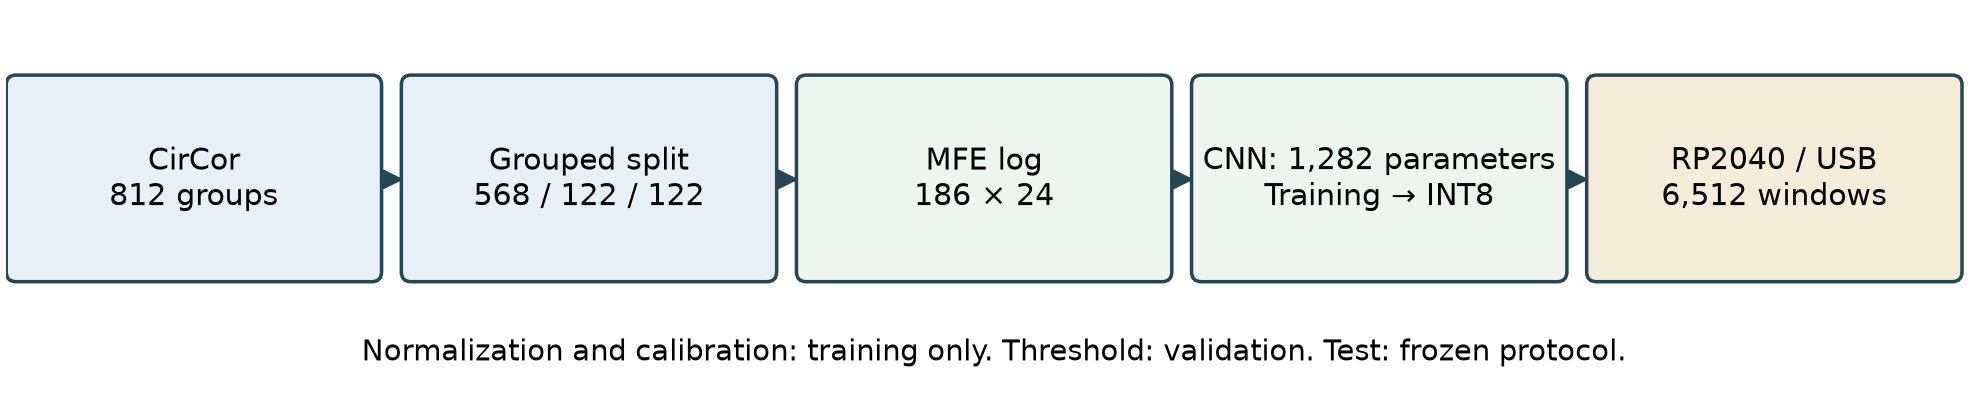
\includegraphics[width=\textwidth]{images/pipeline_en.png}
\caption{Experimental pipeline. Partitioning precedes segmentation and normalization. Model selection and thresholds use validation groups; the RP2040 executes the frozen INT8 model on digitally replayed test inputs.}
\label{fig:pipeline}
\end{figure*}

\section{Related Work}
The CirCor DigiScope dataset provides PCGs and murmur annotations \citep{oliveira2022circor,circor103}. The PhysioNet Challenge 2022 separately evaluated murmur detection and clinical-outcome prediction, including an unknown murmur category \citep{reyna2023challenge}. Our binary subset excludes unknown labels, and its scores are therefore not directly comparable with Challenge rankings or three-class metrics.

For murmur characterization, \citet{elola2023grading} combined mel-spectrogram inputs, an ensemble of residual CNNs, and patient-level aggregation to distinguish absent, soft, and loud murmurs. This supports investigating spectral representations and multi-location aggregation, while differing from our small binary CNN in task, model scale, and evaluation protocol. We do not use that study's scores as a matched benchmark or infer microcontroller execution from its classification results.

TFLM targets inference on memory-constrained devices \citep{david2021tflm}; its integer kernels and platform ports provide a deployment path for compact networks. Quantization specifies tensor scales, zero points, and supported operations \citep{int8spec}. However, numerical agreement must be checked for the selected host and embedded kernels. We explicitly distinguish optimized-host test scores from reference-kernel parity and target execution.
% TODO: ampliar revisao de implementacoes embarcadas somente com protocolos verificados.

\section{Materials and Methods}
\subsection{Dataset and grouped partitions}
We used CirCor DigiScope version 1.0.3, distributed through PhysioNet \citep{circor103,pollard_physionet_2026}. Only \texttt{Murmur = Present} and \texttt{Murmur = Absent} were retained; the clinical \texttt{Outcome} field was not used as the label. The inventory records 68 encounter entries excluded for unknown or missing murmur labels and 31 recording entries excluded for conflicting labels within linked groups. These counts have different units and must not be added as a count of excluded people.

Encounter identifiers were linked using available additional-identity metadata and identical waveform SHA256 hashes. Linked groups were assigned together before segmentation, using approximately 70/15/15\% stratified partitions and split seed 42. Saved assertions verified separation of group identifiers, encounter identifiers, recording identifiers, and waveform hashes. This reduces known identity and duplicate leakage; it cannot establish the absence of unannotated identity links. We refer to these units as patient groups, with this qualification.

The eligible cohort comprises 812 groups and 2,976 recordings (Table~\ref{tab:split}), yielding 28,340 training, 6,154 validation, and 6,512 test windows. Windows inherit the patient murmur label, including recordings at locations where a murmur may be inaudible. This weak supervision precludes treating the inherited labels as verified window-level acoustic annotations.
\begin{table}[t]
\centering
\caption{Achieved grouped partitions. P/A: present/absent groups.}
\label{tab:split}
\begin{tabular}{lrrrr}
\toprule
Partition & Groups & P & A & Recordings\\
\midrule
Training & 568 & 109 & 459 & 2,066\\
Validation & 122 & 24 & 98 & 439\\
Test & 122 & 24 & 98 & 471\\
\bottomrule
\end{tabular}
\end{table}
Test groups contributed one to nine recordings (median four). Test recording counts by metadata location were 119 aortic (AV), 113 pulmonary (PV), 110 tricuspid (TV), and 126 mitral (MV), plus three labeled \texttt{Phc}. The latter were retained without assigning an anatomical interpretation beyond the metadata. This recording inventory is not a count of independently annotated audible murmurs.
% TODO: revisar local Phc no metadado original; nao excluir retrospectivamente pelo resultado.

\subsection{Signal processing}
The loader requires mono PCM16 audio and supports resampling when needed; all 2,976 retained recordings were already sampled at 4 kHz. Three-second windows (12,000 samples) use a 1.5-second hop. Short recordings are zero-padded; incomplete trailing windows in longer recordings are discarded. Each window has its direct-current (DC) component removed.

The front-end uses a periodic 128-sample Hann window, 64-sample frame hop, unnormalized power spectrum, and 24 triangular mel filters spanning 30--1800 Hz. Positive-frequency bins are not doubled. Logarithmic mel-filterbank energies (MFE) are computed as $\log(\max(E,10^{-6}))$, producing a $186\times24$ array. Per-band normalization statistics are fitted only on training features and frozen. The embedded front-end remains floating point; INT8 refers to neural-network tensors. Python and C++ share frozen filter and normalization coefficients, padding, tensor layout, and quantization rounding rules; their observed numerical agreement is assessed separately.


Figure~\ref{fig:examples} illustrates two validation inputs and their spectral representations. The examples were selected by recording identifier within each class, independently of classifier output.
\begin{figure*}[t]
\centering
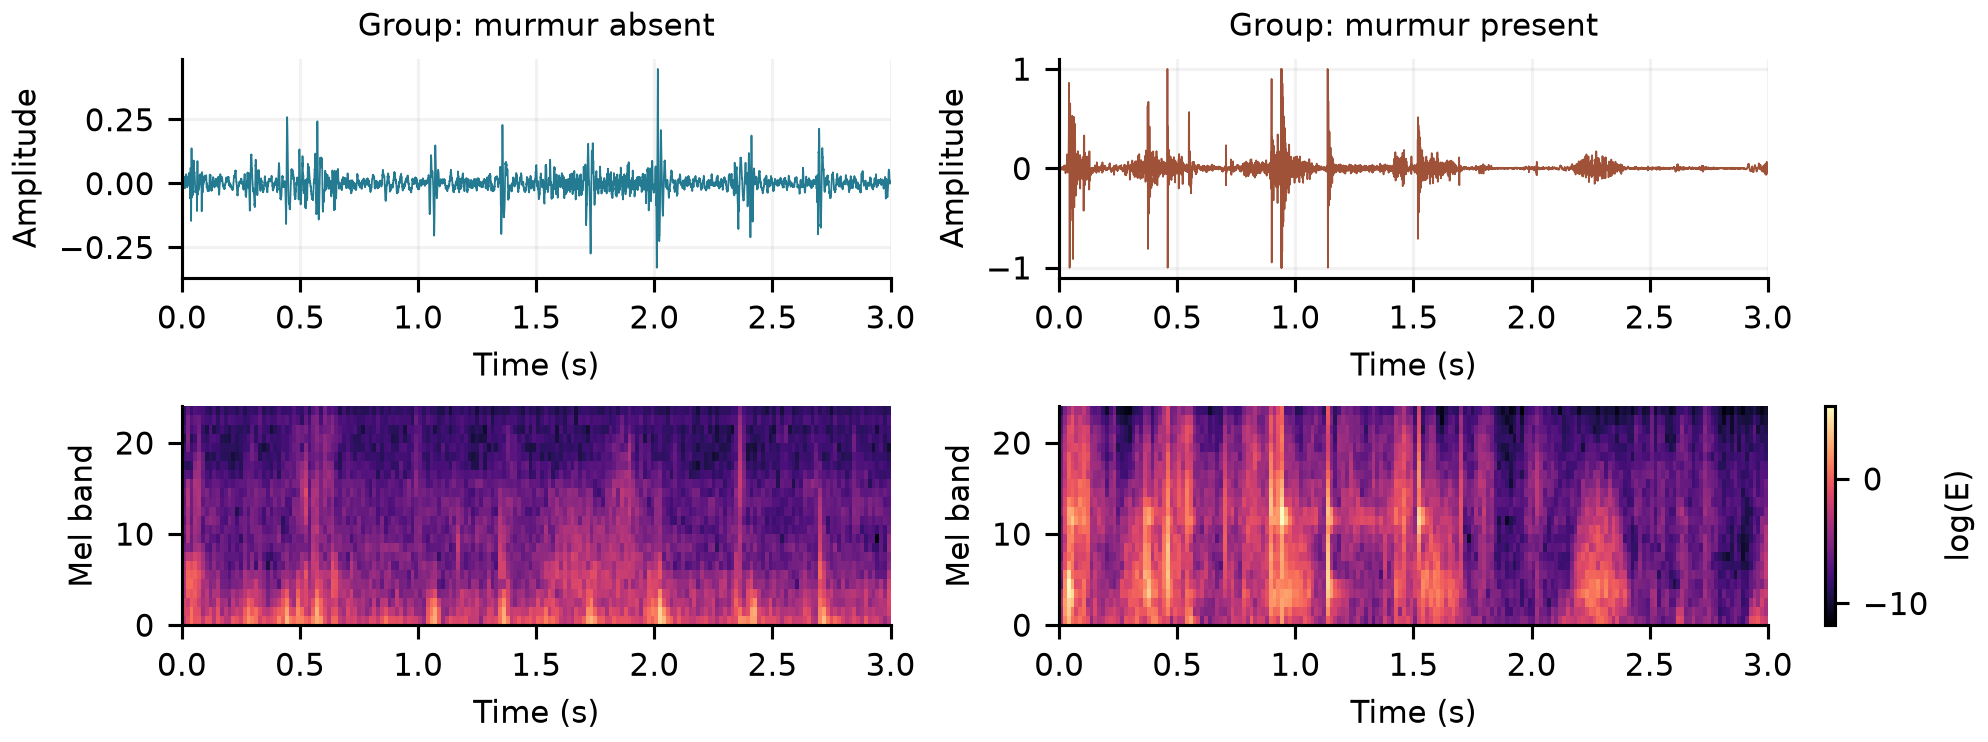
\includegraphics[width=\textwidth]{images/pcg_mfe_en.png}
\caption{Real three-second validation waveforms and corresponding log-MFE from CirCor DigiScope 1.0.3 \citep{circor103}. Each title denotes an inherited group label, not a verified window-level audible murmur. Both spectral images use the same color scale; waveform axes retain their own amplitude ranges.}
\label{fig:examples}
\end{figure*}

\subsection{Network and offline training}
The CNN contains two $3\times3$ convolutions with 8 and 16 channels, each followed by rectified linear unit (ReLU) activation and $2\times2$ max pooling, then global average pooling and a two-class softmax. Convolutions use same padding and unit stride; pooling uses valid padding and stride two. The model has 1,282 trainable parameters.

Training used Adam with learning rate $10^{-3}$, batch size 32, and at most 100 epochs. Early stopping followed ten epochs without a strict improvement in validation patient-level F1. Weighted cross-entropy assigned each window weight proportional to $1/(N_c W_i)$, where $N_c$ is the number of training groups in its class and $W_i$ the group's training-window count; weights were normalized to mean one. No augmentation was used.

Three initializations (seeds 42, 43, and 44) were trained. The highest validation F1 selected seed 43 at epoch 66. The three selected checkpoints had validation F1 of 0.451, 0.711, and 0.618, respectively. These are model-selection results, not repeated test trials. Training ran offline with TensorFlow 2.21 on an RTX 5050 under Arch Linux/WSL; Python, NumPy, and SciPy versions were 3.12.15, 2.0.2, and 1.15.3.

Full-integer post-training quantization used 300 training windows for calibration. The converted graph contains convolution, max pooling, mean, fully connected, and softmax operators, with INT8 input and output. Tensor scales and zero points follow the converter specification \citep{int8spec}. The final serialized model is 5,264 bytes. This single compact architecture was evaluated without an architecture-search or ablation study; its size should not be interpreted as an optimized accuracy--resource frontier.

\subsection{Target implementation}
A C/C++ application embeds the frozen model and executes the MFE front-end and TFLM on the BitDogLab RP2040. The board target is \texttt{pico\_w}; measurements used core 0 at 133 MHz, with no wireless communication or core-1 workload. The RP2040 provides 264 KiB of on-chip SRAM \citep{rp2040docs}. Exact carrier revision was not independently recorded.

Firmware used the Pico software development kit (SDK) commit \texttt{95ea6ac}, the Raspberry Pi TFLM port commit \texttt{dfea53b}, Arm GNU Toolchain 14.2.Rel1, CMake 3.31.6, and Ninja 1.11.1.4. Application compilation used \texttt{-O2}; TFLM used size optimization. Digital PCM16 waveforms were transferred over USB for controlled replay. The BitDogLab project documents microphone and OLED peripherals \citep{bitdoglab}. Microphone acquisition was not implemented, and the benchmark firmware did not drive the display.
% TODO: registrar revisao fisica e medir custos da interface em protocolo separado.

% Demo visual separada: firmware-demo e scripts proprios. Nao atribuir seus custos ao benchmark original.
A separate OLED/RGB demonstrator was subsequently built with two stored validation windows. A manual functional check reported alternating window outputs on the OLED and green/red indications on the RGB LED. These illustrative window outputs do not reproduce patient-level aggregation. This demonstrator is separate from the firmware whose timing and memory are reported here; its additional overhead was not measured.


\section{Experimental Setup}
\subsection{Aggregation and host evaluation}
Window positive-class probabilities are averaged per recording; the patient-group score is the maximum recording score over available locations. A validation threshold maximizes patient F1, breaking ties by higher recall and then lower threshold. The float and INT8 thresholds are 0.725111204844 and 0.734675480769, respectively. The latter is frozen for target testing. Record count and location coverage may affect maximum-score aggregation.

Host testing uses the same 122 held-out groups for a training-majority baseline, float CNN, and INT8 CNN. The original INT8 host evaluation used the AUTO/XNNPACK interpreter. The primary measure is binary patient-level F1, with murmur present positive:
\begin{equation}
F_1=\frac{2TP}{2TP+FP+FN},\qquad R=\frac{TP}{TP+FN}.
\end{equation}
Precision, accuracy, specificity, macro-F1, and raw confusion counts accompany F1. Ordinary patient bootstrap resampling (2,000 replicates, seed 2026) provides percentile 95\% intervals. No model, aggregation, or threshold was selected using test performance.

\subsection{Validation parity and timing}
Before full target-cohort evaluation, ten validation recordings (five per class) were compared against a host interpreter. The validation diagnostic found exact quantized features but optimized-host output discrepancies up to 0.015625 (four output quantization steps). The comparison resolver was then revised to LiteRT 2.3.0 \texttt{BUILTIN\_REF}; model weights, threshold, and tolerances were unchanged. This was a post-diagnostic protocol revision on validation data, and the original AUTO/XNNPACK test results were retained. The revised gate permits at most one input step and two output steps. Reference-compatible integer kernels are a documented concern for Arm deployment \citep{cmsisnn}.

A separate benchmark replayed the first three seconds from each of 100 shuffled validation recordings (NumPy seed 2026), after ten excluded warm-up windows. Firmware timestamps measured front-end and inference duration using \texttt{time\_us\_64}. Acquisition, USB transfer, feature CRC, display, and initialization are outside these intervals. Flash-image bytes were obtained from the linked binary, while SRAM sections were audited from the Executable and Linkable Format (ELF) file. Arena occupancy is reported separately from capacity; peak RAM and stack high-water usage were not instrumented.

\subsection{Full-cohort target test}
The frozen target protocol covered all 6,512 windows from 471 test recordings and 122 groups, retaining input hashes, host comparisons, aggregation, and the INT8 threshold. Each confirmed response was stored in a hash-chained journal. A USB write timeout interrupted the first session after 1,293 windows; evaluation resumed for the remaining 5,219 windows with the same model, sources, and protocol. The physical cause of that interruption was not established.

Metrics were released only after the full cohort was collected. An offline consistency audit verified the response chain and stored artifact hashes and separately recomputed patient aggregation and the primary bootstrap interval. Every test window was included; feature or output disagreements did not trigger filtering or parameter changes.
% Teste completo auditado em docs/full-board-test-audit.json. Nao reexecutar para ajustar ao teste.

\section{Results and Discussion}
\subsection{Predictive performance across runtimes}
Table~\ref{tab:predictive} reports completed host and target results. RP2040 F1 was 0.694 (95\% interval 0.526--0.829), recall 0.708 (17/24 positives), precision 0.680, and specificity 0.918. The original optimized-host INT8 result remains F1 0.680 (interval 0.512--0.816). The target and reference host share all 122 patient decisions; the optimized host differs for one negative group, producing nine rather than eight false positives (Table~\ref{tab:confusion}).

The float CNN and target INT8 run have the same confusion counts, without implying equal probabilities or numerical equivalence. The difference from the optimized INT8 host concerns the combined front-end and runtime implementations under the frozen threshold; it does not isolate a cause or establish an improvement in the underlying model. The small positive cohort produces wide uncertainty intervals.
\begin{table}[t]
\centering
\caption{Completed test results for 122 patient groups. Opt./ref.: optimized/reference host kernels.}
\label{tab:predictive}
\begin{tabular}{lrrrr}
\toprule
Model & F1 & Recall & Accuracy & Macro-F1\\
\midrule
Always absent & 0.000 & 0.000 & 0.803 & 0.445\\
Float CNN & 0.694 & 0.708 & 0.877 & 0.808\\
INT8 host (opt.) & 0.680 & 0.708 & 0.869 & 0.799\\
INT8 host (ref.) & 0.694 & 0.708 & 0.877 & 0.808\\
INT8 RP2040 & 0.694 & 0.708 & 0.877 & 0.808\\
\bottomrule
\end{tabular}
\end{table}
\begin{table}[t]
\centering
\caption{Test confusion counts; present is positive.}
\label{tab:confusion}
\begin{tabular}{lrrrr}
\toprule
Model & TP & FN & FP & TN\\
\midrule
Always absent & 0 & 24 & 0 & 98\\
Float CNN & 17 & 7 & 8 & 90\\
INT8 host (opt.) & 17 & 7 & 9 & 89\\
INT8 host (ref.) & 17 & 7 & 8 & 90\\
INT8 RP2040 & 17 & 7 & 8 & 90\\
\bottomrule
\end{tabular}
\end{table}

The majority baseline achieves 80.3\% accuracy while detecting no positive cases, illustrating why accuracy alone is inadequate for this cohort. Its precision is undefined. The INT8 model still misses seven of 24 positive groups. These observations, the binary exclusion of unknown labels, weak window labels, and the absence of external validation limit clinical interpretation. The model is a research prototype, not a clinically validated diagnostic system.


Figure~\ref{fig:results} combines the target confusion matrix, patient-bootstrap uncertainty, and measured processing costs. Its intervals describe patient-level predictive uncertainty; its latency bars summarize all 6,512 test windows.
\begin{figure*}[t]
\centering
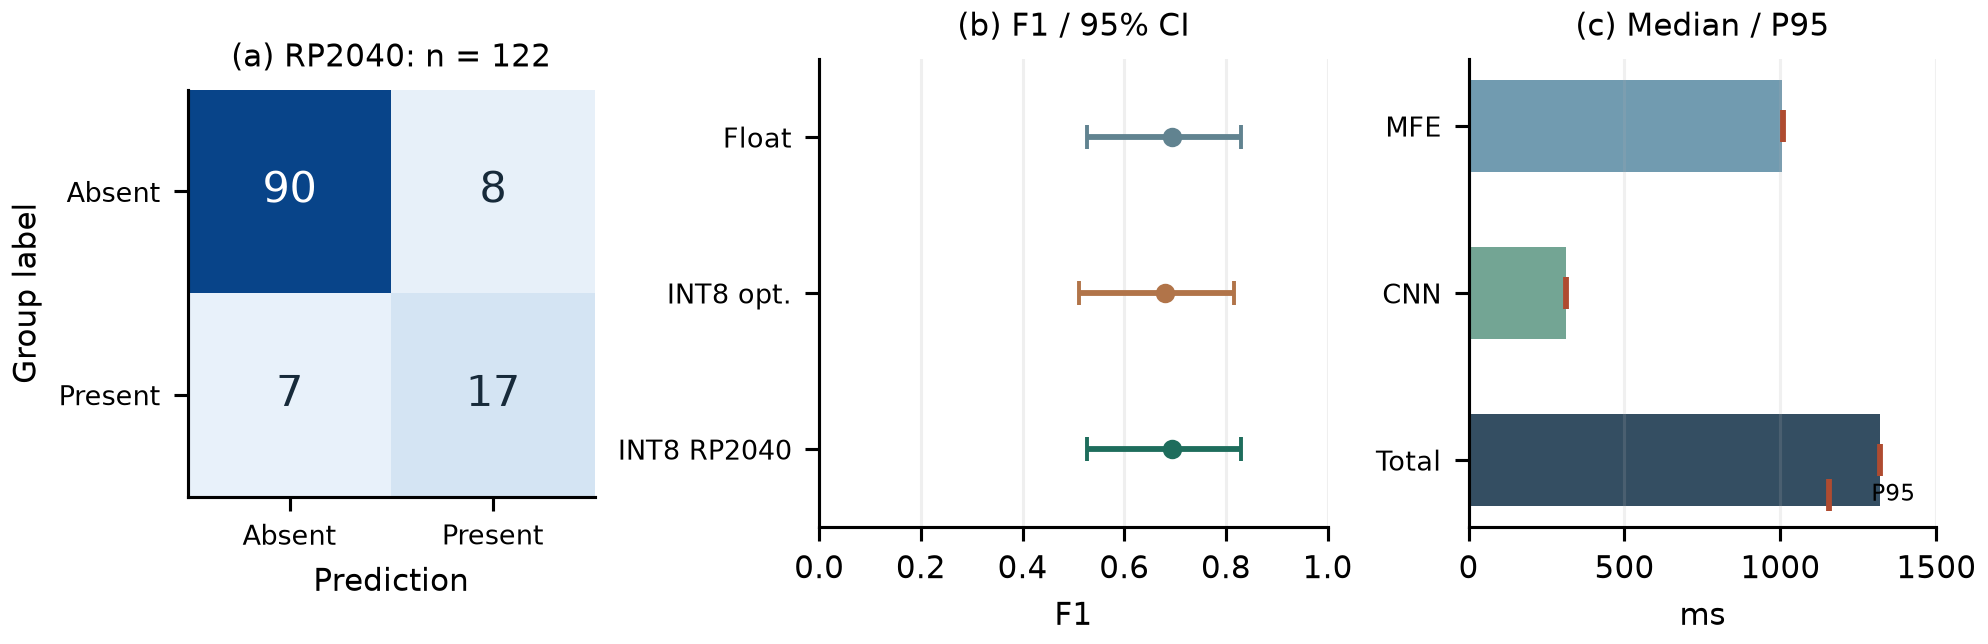
\includegraphics[width=\textwidth]{images/results_en.png}
\caption{Completed test results: (a) RP2040 confusion counts for 122 groups; (b) F1 and 95\% patient-bootstrap intervals; (c) median processing duration with P95 markers. Timing excludes acquisition, USB, CRC, display, and initialization. The optimized-host INT8 result is kept distinct from the target.}
\label{fig:results}
\end{figure*}

\subsection{Measured target resources}
Table~\ref{tab:resources} distinguishes storage and memory quantities. The arena's 46,100-byte reported occupancy is part of its 147,456-byte static reservation and must not be added to static RAM again. The 186,224-byte static main-SRAM span includes copied code/data, vectors, BSS, and alignment. It excludes heap and stack reservations; it is not peak runtime RAM. Minimum heap reservation is 2,048 bytes, with separate 4,096-byte stack reservations for each core, although core 1 is not executing the application.
\begin{table}[t]
\centering
\caption{Target resource accounting. Values in bytes.}
\label{tab:resources}
\begin{tabular}{p{0.66\columnwidth}r}
\toprule
Quantity & Bytes\\
\midrule
Serialized INT8 model & 5,264\\
Firmware flash image & 189,408\\
Static main-SRAM span & 186,224\\
Tensor arena capacity (included above) & 147,456\\
Tensor arena occupancy (within capacity) & 46,100\\
PCM buffer (included above) & 24,000\\
Runtime peak RAM / stack high-water & \pending\\
\bottomrule
\end{tabular}
\end{table}

\subsection{Numerical agreement on the complete test set}
All 44,640 quantized feature elements across the ten validation inputs matched the host exactly, with zero reference-output difference. The full test set did not extend this to bit-exact agreement: 86 of 6,512 windows (1.32\%) had different 32-bit cyclic redundancy check (CRC32) values for their quantized features. Feature dumps were not retained for those target test inputs, so the cause and element-wise magnitude cannot be established from the saved journal. A feature-checksum difference is not, by itself, evidence of corrupted USB payloads.

Output probabilities differed from reference-host values in 160 test windows; the maximum absolute difference was 0.0078125, or two output quantization steps. Despite these differences, all 122 patient decisions agreed with the reference host. Agreement with the optimized host was 121/122, and its maximum window-output difference from the target was 0.078125. These results distinguish task-level reproducibility from feature- or output-level equivalence. The discrepancy is retained as a limitation rather than corrected using the test set.
% TODO: investigar diferencas do front-end em protocolo separado, sem ajustar pelo teste.

\subsection{Full-test processing latency}

Table~\ref{tab:timing} reports timing for all 6,512 target test windows, excluding validation checks and warm-ups repeated at session startup. Median front-end duration was 1,006.536 ms versus 311.868 ms for inference; feature extraction dominates combined processing. The maximum combined time, 1,323.475 ms, was below the 1,500 ms window hop across this replayed test set. This leaves a measured compute margin under the benchmark conditions, but does not demonstrate continuous real-time operation because acquisition, transfer, and other overheads were excluded. No floating-point model was timed on the target, so these measurements do not quantify an INT8 speedup relative to target float inference.
\begin{table}[t]
\centering
\caption{RP2040 full-test replay timing, 6,512 windows; milliseconds. Validation checks and warm-ups excluded.}
\label{tab:timing}
\setlength{\tabcolsep}{4pt}
\begin{tabular}{lrrr}
\toprule
Stage & Median & P95 & Maximum\\
\midrule
MFE front-end & 1,006.536 & 1,008.025 & 1,011.607\\
Inference & 311.868 & 311.884 & 312.178\\
Combined & 1,318.405 & 1,319.889 & 1,323.475\\
\bottomrule
\end{tabular}
\end{table}
% TODO: medir pico de RAM e watermark da pilha com instrumentacao no hardware.
% Resultados completos conferidos com o diario e os relatórios congelados.

\subsection{Reproducibility and remaining evidence}
The retained artifacts include the inventory and grouped split manifest, training histories, export receipt, original host predictions, linked-firmware audit, and target USB journals. The deployed model has SHA256 prefix \texttt{3b7e258e26ca}; the full digest and source-file hashes are recorded in the receipts. These artifacts are retained locally; a public code archive has not been released. No new participant recordings were acquired in this study.

The original host evaluation, validation benchmark, and completed target test are fixed evidence sets. Resuming the target protocol preserved weights, thresholds, sample order, and comparison tolerances. Additional acoustic, numerical-diagnostic, or memory experiments require separate recorded configurations and cannot be inferred from the existing digital replay. No test-based changes to the model, aggregation, or decision threshold were made.
% TODO: disponibilizar codigo e protocolo com versao/licenca, sem publicar dados pessoais.
% TODO: inserir link publico real somente depois da publicacao autorizada do repositorio.

\section{Conclusion}
A 1,282-parameter CNN quantized to a 5,264-byte model achieved patient-level F1 of 0.694, recall of 0.708, and accuracy of 0.877 during complete held-out replay on a BitDogLab RP2040. Target and reference-host decisions agreed for all 122 groups; feature and output differences nevertheless prevent a claim of bit-exact equivalence. Median combined processing was 1.318 seconds over 6,512 test windows, supporting controlled replay feasibility. Wide predictive uncertainty, unresolved front-end differences, unmeasured peak RAM, and the absence of acoustic and streaming validation limit the result. Further work should address these limitations with separately recorded experiments rather than retuning on this test set.

\bibliographystyle{abbrvnat}
\bibliography{references}
\end{document}


